\chapter{级联闭锁自适应方向保护原理}

为了对各种配电网结构都具有适应性,能支持支持开环和闭环多种运行方式,能适应配电网工作于孤岛、并网两种模式,本章研究基于自适应级联方向闭锁原理的配电网电流保护方案;采用本方案后,无需额外配置专门的母线保护,能够快速切除母线故障,避免扩大停电范围。与差动保护相比,本保护方案具有更优的经济性,适合在主动配电网中大量采用。

\section{有源配电网保护研究的发展}

如第一章所述,传统的配电网保护难以适应配电网的新变化。为此,研究者提出了多种新型保护方案。根据保护方案是否依赖于通信技术,可将已提出的智能配电网保护方案分为两大类。

第一类保护方案仅利用站内信息。由于不依赖通信,故在可靠性与成本方面有明显优势。文献\cite{dewadasa2010fold}和\cite{wentao2014wei}分别提出了反时限导纳和低阻抗保护原理。但由于配电网地理区域小、线路短,使得无论采用电压、电流、阻抗或导纳等作为特征量,定值配合都非常困难。文献\cite{zamani2011protection,najy2013optimal,hsieh2014adaptive,zeineldin2015optimal}基于方向元件和过电流元件,构成了能够适应DG接入的微网和配电网保护方案。但是,文献\cite{zamani2011protection}仅适应于开环运行的辐射型网络,且保护的选择性主要依靠保护之间逐级延时配合实现,导致总体动作速度较慢;文献\cite{najy2013optimal}的方案仅针对同步电机型DG做了仿真分析,且需要故障限流器的配合;文献\cite{hsieh2014adaptive,zeineldin2015optimal}采用反时限过电流保护的逐渐配合原理,整定配合非常复杂,且总体动作速度较慢。此外,文献\cite{ganzhong2002shu}在仅利用线路单端电气量的无通道保护方案方面进行了探索。但所提出的系统不平衡度原理不适用于对称性故障,而电流二次突变量原理又存在整定困难。所以,该方案的自适应性与可靠性仍需做进一步研究。

另一类保护方案需要依赖通信。根据所通信信息的类型,又可以分为两种。一种需要通信模拟量的信息,比如数字式的差动保护\cite{qing2014recent}。但这种方法需要传输的信息量极大,需要解决克服大量信息实时通信特有的问题,比如同步问题、带宽问题等等,离实际应用还有相当大的距离。另一类仅需交换逻辑量的信息,比如故障方向的判断结论。由于传输的信息量不大,对通信带宽要求低,而且不需要同步采样,这种方案更有希望实际应用于有源配电网。文献\cite{wangwei2009}提出了区域纵联方向保护方案,采用一主多从的系统架构。但在这个方案中,一旦保护主机发生故障,整个保护系统都不能正常运行。

\subsection{级联闭锁电流保护方案}

在不含DG的辐射型配电网中,如图\ref{fig:interlocking}所示的级联闭锁保护方案早已被采用\cite{yong1990optimizing},闭锁信号利用屏蔽双绞线级联传输,闭锁方向固定由负荷侧指向电源侧(系统侧)。设F点发生故障,则保护PR4~PR1的过电流保护都起动并向上游保护发送闭锁信号。保护PR5因感受不到故障电流而不发闭锁信号。最终,保护PR4因收不到闭锁信号而动作切除故障。可见,该方案对于传统辐射型配电网具有明确的选择性。

\begin{figure}[!htp]
  \centering
  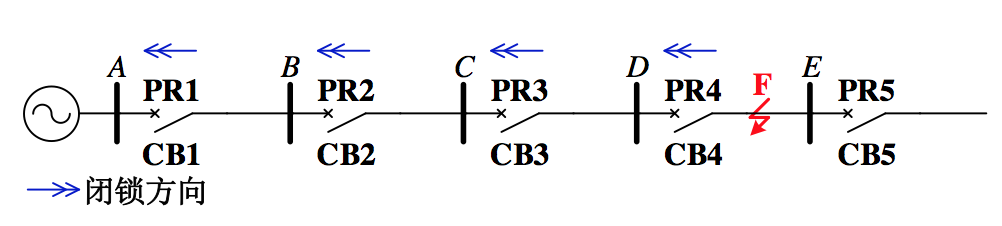
\includegraphics[width=0.6\textwidth]{chap2/interlocking}
  \bicaption[fig:interlocking]{级联闭锁电流保护方案}{级联闭锁电流保护方案}{Fig.}{Interlocking overcurrent protection schema}
\end{figure}

上述级联闭锁方案中不配置方向元件,因而当配电网含有DG或采用闭环拓扑时将失去选择性。为此,文献\cite{libin2010han}提出为电流保护增加方向元件,构成适合闭环配电网的级联方向闭锁纵联电流保护方案。例如在图\ref{fig:interlocking}中,在为电流保护增加方向元件后,在具有相同参考方向的一组保护中,如PR1~PR5,就可以继续采用上述级联闭锁方案。但该方案不具备母线保护功能,母线故障需要依靠相邻变电站切除。例如,变电站D的母线故障需要变电站C、E的保护动作切除。

\subsection{级联方向闭锁电流保护方案}

对于环型供电网络,或者接入了DG的辐射型配电网,文献\cite{oudalov2009adaptive}提出了另外一种针对含DG配电网的级联方向闭锁保护方案,在受影响的保护处增加方向元件,从而将保护分为两组,如图\ref{fig:directional}所示。与文献\ref{libin2010han}采用固定闭锁方向所不同的是,其闭锁方向会随着故障点的不同而自适应改变,克服了上一方案的缺点。但该文提出的方案同样不具备母线保护功能,且不能适应闭环配电网。但本方案不具备母线保护功能,母线故障需要依靠相邻变电站切除。例如,变电站D的母线故障需要变电站C、E的保护动作切除。另外,该文对所提出的保护方案缺乏具体实现方案和分析验证。

\begin{figure}[!htp]
  \centering
  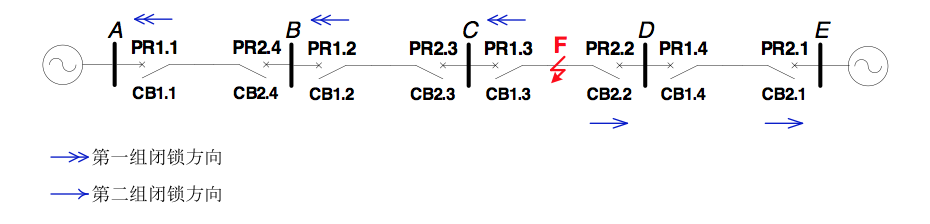
\includegraphics[width=0.6\textwidth]{chap2/directional}
  \bicaption[fig:directional]{级联方向闭锁电流保护方案}{级联方向闭锁电流保护方案}{Fig.}{Directional interlocking overcurrent protection schema}
\end{figure}

方向闭锁原理能够实现线路故障的全线速动,同时无需同步采样且对通信带宽要求低,故较之差动保护具有更好的经济性。文献\cite{liukai2014zhu,nikolaidis2016communication,libin2010han}提出了几种方向闭锁纵联电流保护方案,其中,文献\cite{liukai2014zhu,nikolaidis2016communication}针对辐射形配电网,而文献\cite{libin2010han}则适合闭环运行配电网。但这些方案仅具备线路保护功能,而在配电网中,母线故障概率较高,且易造成开关设备烧毁,甚至烧坏直流操作回路造成整站保护拒动。但中低压母线一般不设专门的母线保护,母线故障需靠相邻线路保护切除,动作时间较长,并且往往要扩大停电范围。

在以上原理的基础上,本文提出的自适应级联方向闭锁电流保护方案同时具备快速线路和母线保护功能,且能适应开环和闭环等多种配电网结构。

\section{面向环形配电网的自适应方向保护方案}

\subsection{方向闭锁保护原理}

图\ref{fig:schematic}为本保护方案的原理示意图,图中每套保护(Protective Relay,PR)由方向元件和启动元件组成。

\begin{figure}
    \centering
    \subfigure[配电网正常运行]{
        \begin{minipage}[b]{0.5\textwidth}
        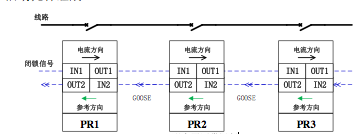
\includegraphics[width=1\textwidth]{chap2/schematic_a}
        \label{fig:schematic_a}
        \end{minipage}
    }
    \subfigure[故障后新的闭锁方向]{
        \begin{minipage}[b]{0.5\textwidth}
        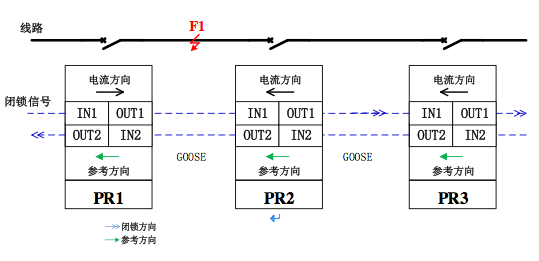
\includegraphics[width=1\textwidth]{chap2/schematic_b}
        \label{fig:schematic_b}
        \end{minipage}
    }
    \bicaption[fig:schematic]{自适应方向保护原理示意图}{自适应方向保护原理示意图}{Fig.}{Schematic of adaptive directional protection}
\end{figure}

保护的参考方向设置为$PR3 \to PR2 \to PR1$,如图\ref{fig:schematic} \subref{fig:schematic_a}。当F1处发生故障时,PR1、PR2、PR3的过流元件皆起动,PR1判别出故障方向异于参考方向,而PR2、PR3的故障方向同于参考方向,如图\ref{fig:schematic} \subref{fig:schematic_b}。为正确切除故障,PR1需要顺着参考方向发送闭锁信号,而PR2、PR3则需逆参考方向发送闭锁信号。这样,F1处故障才可以被保护PR1、PR2选择性切除,而其余保护则被闭锁。

原理的保护跳闸条件为本地过流保护起动,并且未收到闭锁信号。判据如下:

\begin{equation}
    \label{eq:trip}
    Trip = NOT (BlockingSignal) AND (I>I\_set) 
\end{equation}}
	 
式\ref{eq:trip}中,$BlockingSignal$指收到的闭锁信号,$I\_set$为本地过流保护起动定值,按躲最大负荷整定。

利用GOOSE交换闭锁信号,可以大量减少控制电缆,提高保护之间的互操作性。同时,还可以充分利用GOOSE的通信自检机制,提高保护的可靠性。根据GOOSE的收发原理,在图2中,每套保护设置了两组、四个GOOSE虚端子。其中,第一组虚端子IN1、OUT1负责逆参考方向闭锁信号的接收与发送;第二组虚端子IN2、OUT2则负责顺参考方向闭锁信号的收发。在智能配电网中,可以根据不同需要,选择光纤、电力线甚至无线网络等多种介质\cite{huangfei2013ji,parikh2013comprehensive,kanabar2009evaluation}完成GOOSE的收发。

\subsection{参考方向和闭锁方向规则}

由上可见,为了保证自适应方向保护方案的选择性,需要建立参考方向和闭锁方向的相关规则。

以图\ref{fig:cankao}所示的典型环型和辐射型配电网为例,本文定义如下参考方向的整定规则:

\begin{figure}
    \centering
    \subfigure[环型配电网]{
        \begin{minipage}[b]{0.5\textwidth}
        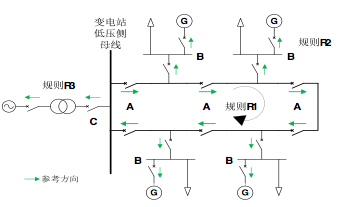
\includegraphics[width=1\textwidth]{chap2/cankao_a}
        \label{fig:cankao_a}
        \end{minipage}
    }
    \subfigure[环型配电网]{
        \begin{minipage}[b]{0.5\textwidth}
        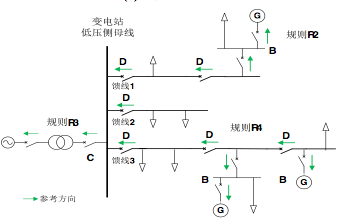
\includegraphics[width=1\textwidth]{chap2/cankao_b}
        \label{fig:cankao_b}
        \end{minipage}
    }
    \bicaption[fig:cankao]{参考方向整定规则示意图}{参考方向整定规则示意图}{Fig.}{Schematic of rules of reference directions}
\end{figure}

\textbf{R1}:环网中馈线断路器(图\ref{fig:cankao}中A所示)的参考方向为沿环同向,即同沿顺时针或逆时针方向;

\textbf{R2}:分支线断路器(图\ref{fig:cankao}中B所示)的参考方向为远离主电网方向;

\textbf{R3}:配电变电站断路器(图\ref{fig:cankao}中C所示)的参考方向为指向主电网方向;

\textbf{R4}:辐射型馈线断路器(图\ref{fig:cankao}中D所示)的参考方向为指向主电网方向。

此外,本文定义了如下闭锁方向规则:

\textbf{B1}:若故障电流与参考方向同向,则闭锁方向与参考方向反向。闭锁信号由IN1、OUT1收发;

\textbf{B2}:否则,则闭锁方向与参考方向同向。闭锁信号由IN2、OUT2收发。

上述规则可以用两种基本故障类型加以解释,如图\ref{fig:two}所示。当发生线路故障时,全系统只有F1点呈现图\ref{fig:two} \subref{fig:two_a}所示的汇流特征,导致只有F1点两侧的保护闭锁方向相背,最终仅保护PR1、PR2因收不到闭锁信号而动作,线路故障F1被选择性切除;当发生母线故障时,全系统只有F2点呈现图\ref{fig:two} \subref{fig:two_b}的汇流特征,最终只有保护PR1~PR3因收不到闭锁信号而动作,母线故障F2被选择性切除。

\begin{figure}
    \centering
    \subfigure[线路故障]{
        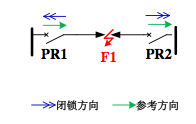
\includegraphics[width=0.3\textwidth]{chap2/two_a}
        \label{fig:two_a}
    }
    \hspace{1in}
    \subfigure[母线故障]{
        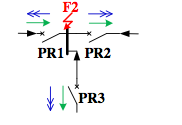
\includegraphics[width=0.3\textwidth]{chap2/two_b}
        \label{fig:two_b}
    }
    \bicaption[fig:two]{两种基本故障类型}{两种基本故障类型}{Fig.}{Two primary fault types}
\end{figure}


\subsection{保护的功能逻辑图}

自适应方向保护方案的实现逻辑如图\ref{fig:logic}所示。

\begin{figure}[!htp]
  \centering
  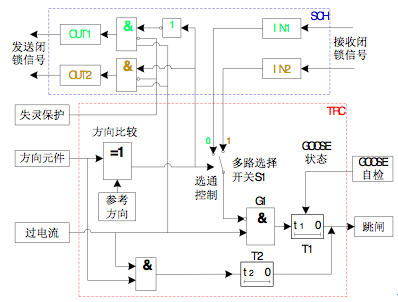
\includegraphics[width=0.6\textwidth]{chap2/logic}
  \bicaption[fig:logic]{自适应方向保护方案的逻辑图}{自适应方向保护方案的逻辑图}{Fig.}{Logic diagram of adaptive directional protection}
\end{figure}

SCH功能块(图中上部虚线框内)实现方向闭锁信号的收发功能。IN1/2、OUT1/2分别对应于图2中保护的两组GOOSE虚端子。

TRC功能块(图中下部虚线框内)根据式(1)实现跳闸条件综合判别功能。首先由方向元件判别故障方向,然后由方向比较模块将其与参考方向比较。如果同向则执行规则B1,此时方向比较模块输出0,控制多路选择开关S1选通端子IN1,并经反相器向OUT1输出闭锁信号;如果反向则执行规则B2,此时方向比较模块输出1,开关S1选通IN2,并向OUT2输出闭锁信号。考虑到闭锁信号的延时,以及相邻保护的起动和返回时间的不一致性,增加了延时动作元件T1。考虑到GOOSE发送延时应小于3ms\cite{baigent2004iec},以及配电网线路较短等因素,延时时间t1可整定为20~100ms。

对于闭锁原理,如果通信失效后发生区外故障,保护会因收不到闭锁信号而误动\cite{shengshi1981}。为解决这个问题,在图5中,利用GOOSE的自检机制,可在1s左右探测到通信失效,并自动增大t1定值(如增大至0.6s)以防止保护误动,同时发送告警信号。当外部故障被切除后,本保护瞬时返回。

如果区内故障但断路器失灵,失灵元件动作并输出1,经反相后闭锁OUT1、OUT2的输出。这样,沿闭锁方向的上一级保护因收不到闭锁信号而以近后备或远后备方式动作并切除故障。

如果下游保护拒动,本方案利用图\ref{fig:logic}中的时间元件T2提供后备保护回路。T2串联在过流元件之后,其时间定值以解环点按照逐级配合原则整定,以传统的定时限过电流方式提供可靠的后备功能。

\subsection{环型配电网中保护动作情况分析}

上节提出一种自适应方向保护方案。该方案同时具备线路和母线保护功能,能够实现配电网全范围故障的快速动作。但从保护可靠性角度,上述方案依旧存在两点不足:

\begin{enumerate}
    \item 当配电网开环运行时,故障点下游保护的短路电流仅由DG提供,属于弱溃系统,其起动元件和方向元件的灵敏度不足;
    \item 电流保护作为起动元件,按躲开最大负荷考虑,配电网故障时,非故障线路的保护仅靠方向元件闭锁,对方向元件的依赖很大,存在误动的可能性。
\end{enumerate}

而且该方案主要针对闭环运行的配电网,而目前配电网仍主要采用开环运行的方式。此外,该文献对配电网重构讨论不足。

本文在上一节的基础上,针对更具代表性的开环运行的主动配电网,根据其树状拓扑结构特点,提出一种原理简单的继电保护方案进一步做出两点改善:

\begin{enumerate}
    \item 线路一侧保护动作时,同时向对侧保护发出联跳信号,从而解决对侧弱溃问题;
    \item 电流保护采用两段配置。其中,\uppercase\expandafter{\romannumeral1}段保护范围为本线路全长,为主电流保护;\uppercase\expandafter{\romannumeral2}段保护范围为相邻线路全长,为后备电流保护。
\end{enumerate}

这样,当配电网发生故障时,仅故障点相邻线路的电流保护会起动,有效减少对方向元件正确性的依赖。该方案具备对短路电流水平的适应性、对拓扑结构改变的适应性以及对不同故障元件的适应性。本方案的原理如图5-4所示。


\section{面向辐射形配电网的改进型保护方案}

\section{本章小结}